\subsection{RQ1 \textemdash{} Guardrail Effectiveness}

% Report error/warning counts before and after the guardrail, per model and per prompt. Show whether the guardrail improves semantic correctness — and be careful to distinguish between W3C validation errors and semantic correctness (flag this distinction explicitly here).

% \textbf{Change}: Results now need to be broken down by condition (\verb|feedback| vs \verb|blind|) as well as by model and difficulty tier, not just before/after. The statistical analysis uses paired Wilcoxon tests and 95\% confidence intervals, which should be stated. Also add error category breakdown as a dimension (missing-doctype, stray-tag, disallowed-attribute, etc.).

% = PARAGRAPH 1 = Measurement caveat upfront

Before presenting any numbers, restate the key distinction from Section 4.4: W3C error/warning counts are your primary metric, but they are a proxy for semantic correctness, not a direct measure of it. Flag this explicitly here so the reader interprets what follows with the right expectations. One short paragraph, load-bearing for the integrity of the section.

% = PARAGRAPH 2 = Overall before/after results (feedback condition)

Present the aggregate picture first: total error and warning counts before and after the guardraila cross all models and all 51 prompts, in the \verb|feedback| condition. Introduce your primary summary table here (errors before/after, warnings before/after, delta, percentage reduction). State the result of the paired Wilcoxon test and 95\% confidence interval -- does the guardrail produce a statistically significant reduction in errors?

% Primary summary table: see tables.tex, Table~\ref{tab:rq1-aggregate} (tab:rq1-aggregate).
% Per-model breakdown (supplementary to the aggregate number above):
\begin{figure}[H]
	\centering
	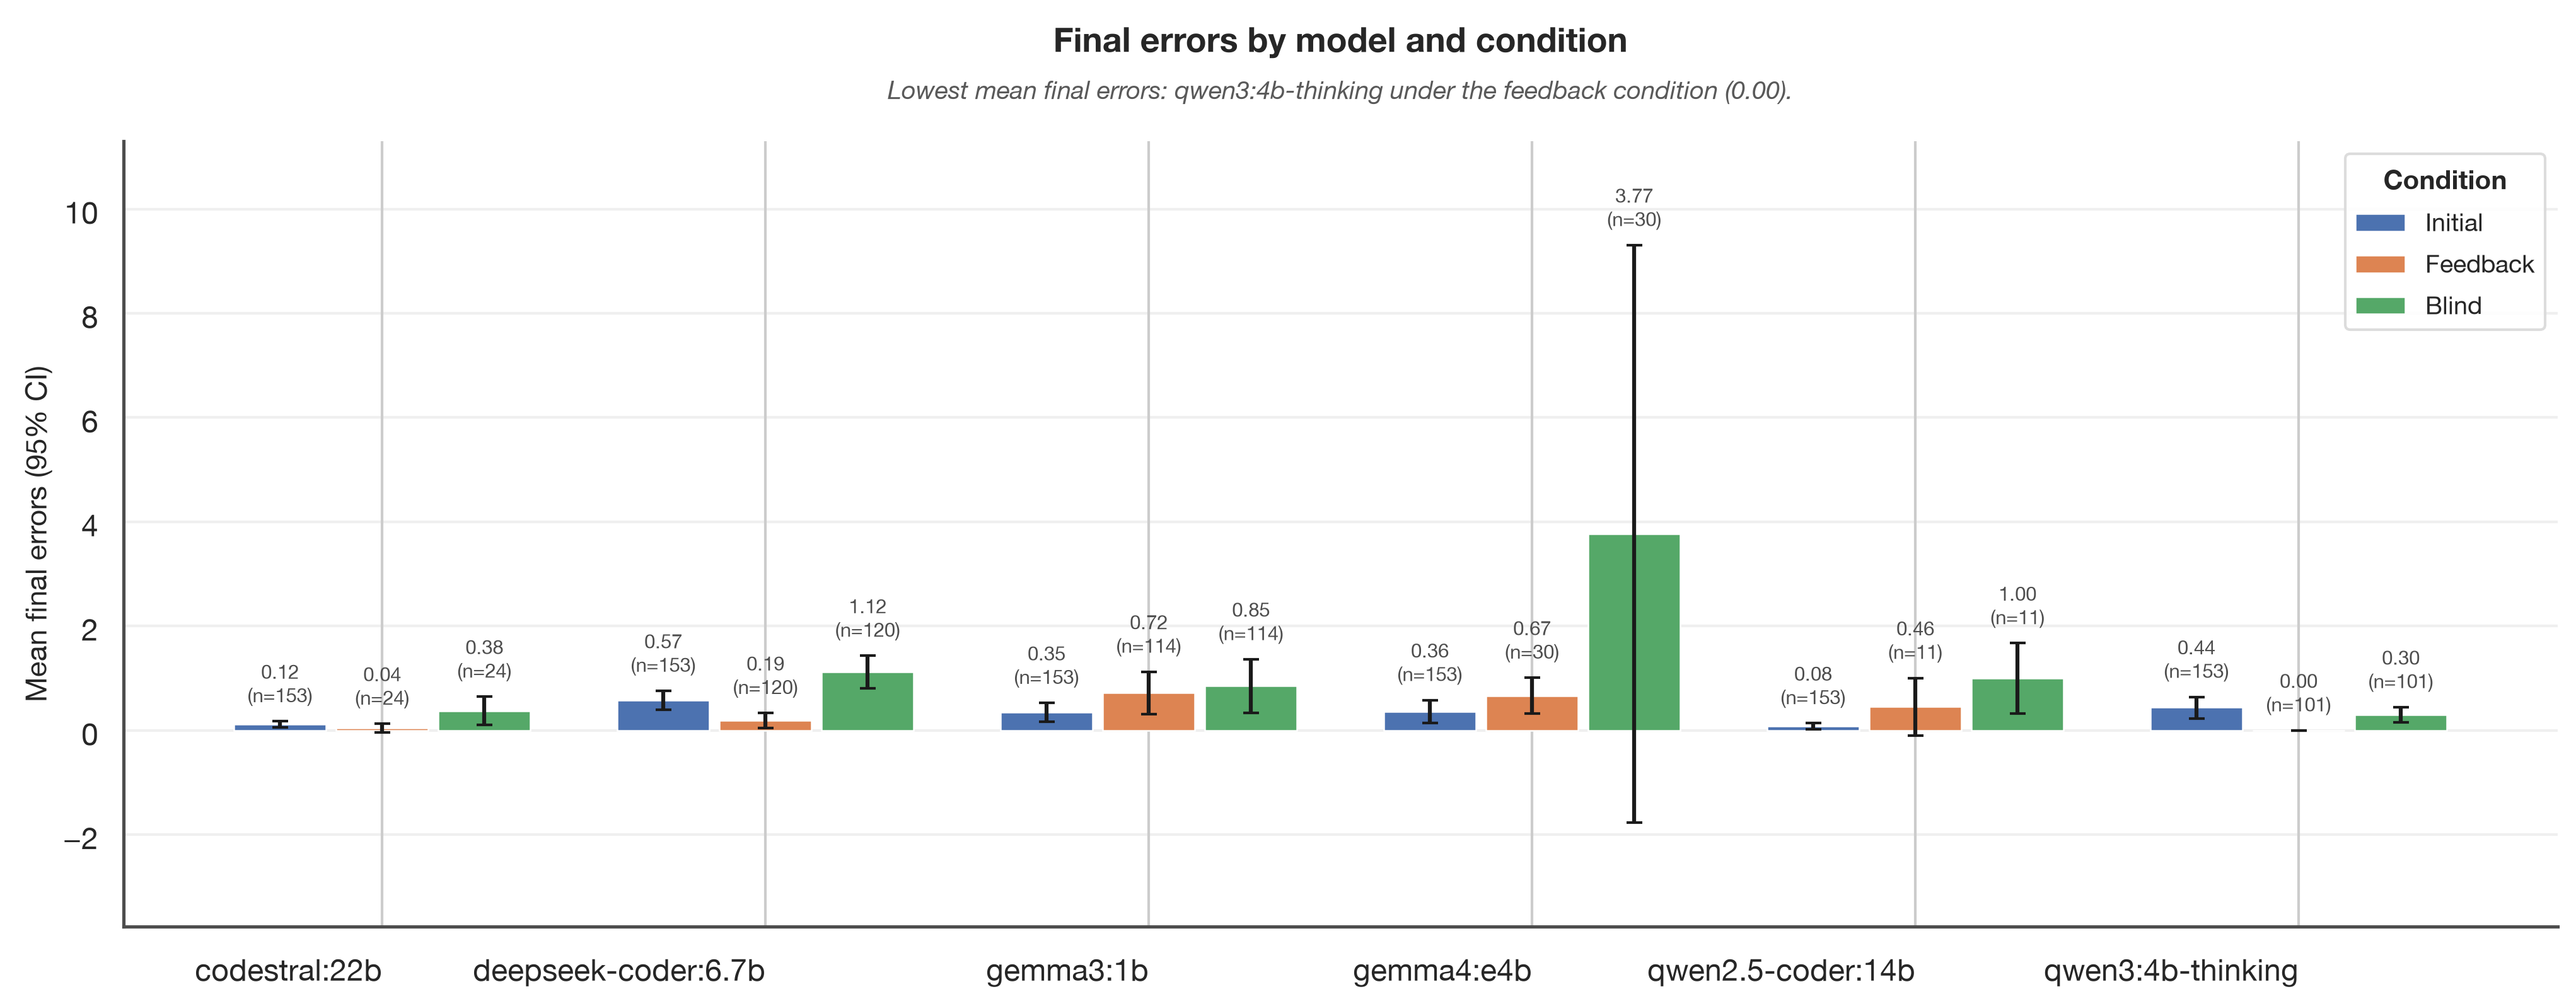
\includegraphics[width=\linewidth]{images/final_summary_errors.png}
	\caption{Mean final error count (95\% CI) by model and condition (initial / feedback / blind). Value and $n$ are annotated above each bar since several models converge to exactly zero.}
	\label{fig:final-summary-errors}
\end{figure}

% = PARAGRAPH 3 = Feedback vs. blind condition

Now introduce the ablation comparison. How does the \verb|feedback| condition compare to the \verb|blind| condition in terms of error reduction? This is the central validity argument for your guardrail design. If the \verb|feedback| condition significantly outperforms \verb|blind|, it means the validator's specific error list is doing real work, not just the act of reprompting. Present this as a table or figure comparing mean error reduction across both conditions, with statistical test results. I think I can split this up by difficulty of the prompt, for reasoning and non-reasoning models combined (2 categories) -> so 2 columns and 6 rows.

% Difficulty x reasoning-category ablation table: see tables.tex, Table~\ref{tab:rq1-feedback-vs-blind-reasoning} (tab:rq1-feedback-vs-blind-reasoning).
\begin{figure}[H]
	\centering
	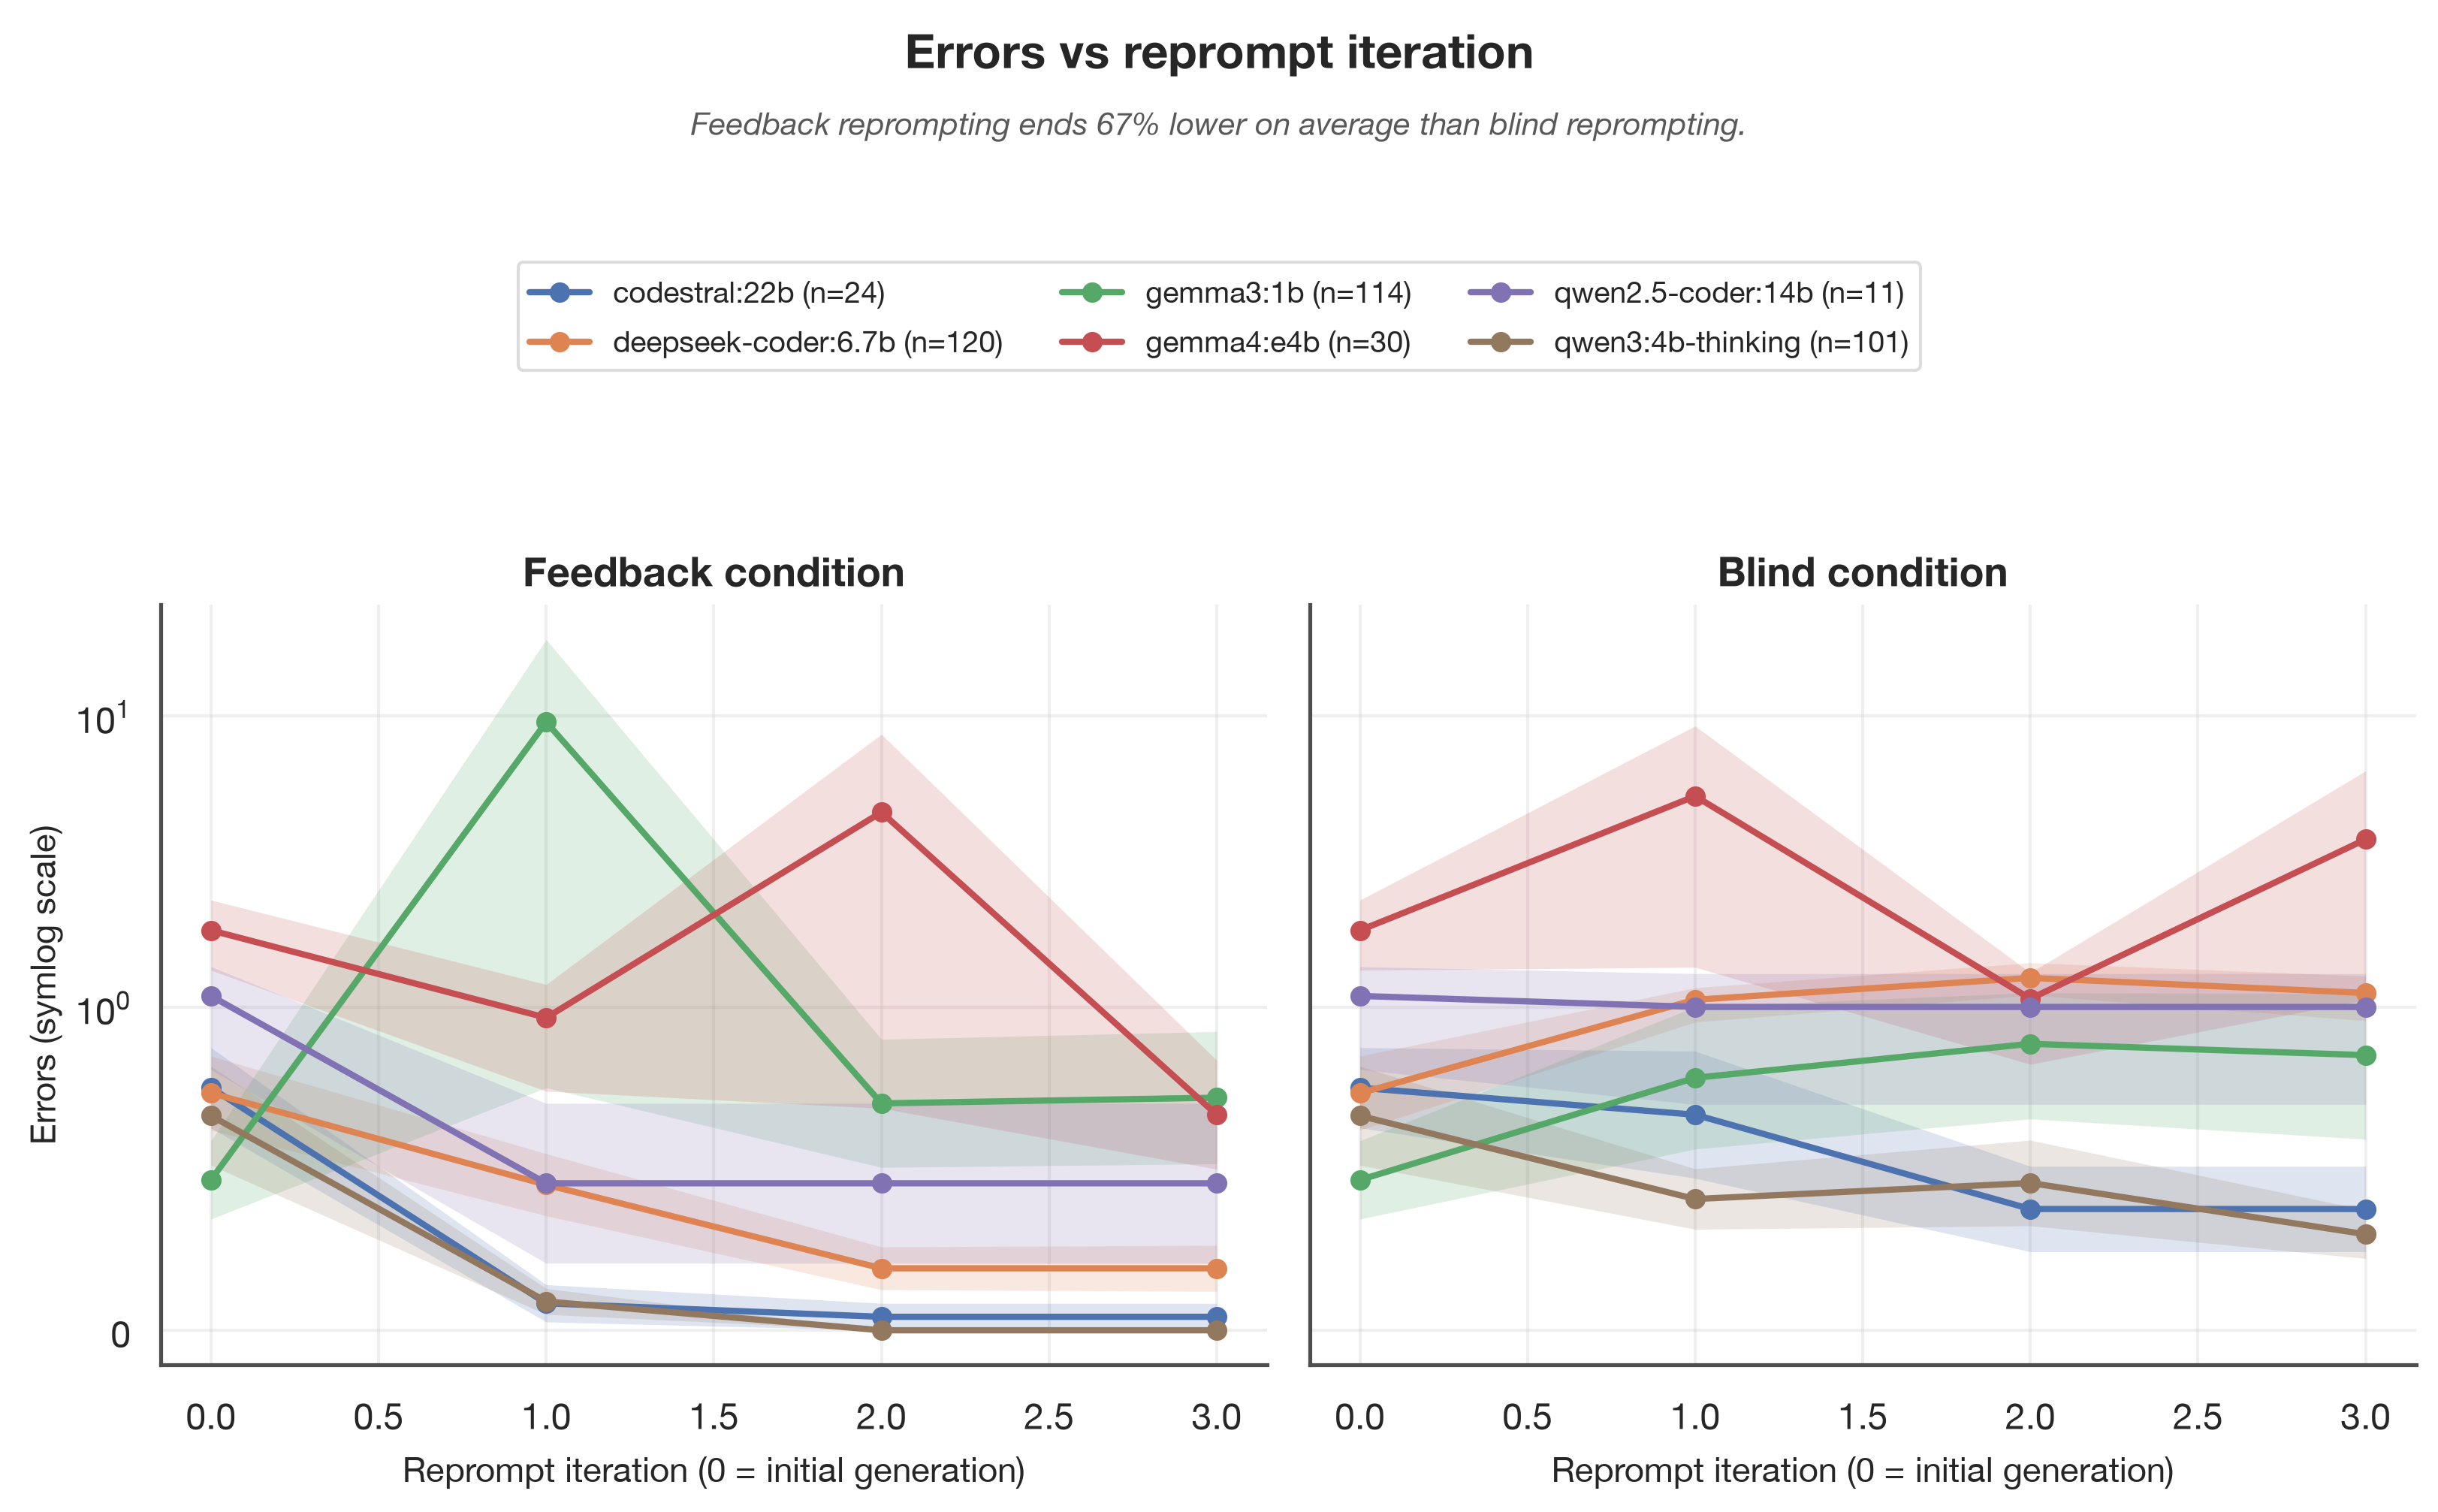
\includegraphics[width=\linewidth]{images/trajectory_errors.png}
	\caption{Mean error count per reprompt iteration, one line per model, feedback vs blind condition (shaded band = $\pm 1$ SEM; symlog $y$-axis since per-model means span roughly 0--60 errors). Feedback and blind start from the same iteration-0 (initial) generation.}
	\label{fig:trajectory-errors}
\end{figure}

% = PARAGRAPH 4 = Breakdown by difficulty tier

Discuss whether error reduction varies across simple / medium / difficult prompts. You would expect harder prompts to have higher starting error counts (because they simply have more lines of code to make a mistake in) and potentially require more iterations to converge -- confirm or challenge this expectation with your data. A grouped bar chart per difficulty tier (before/after, per condition) works well here.

\begin{figure}[H]
	\centering
	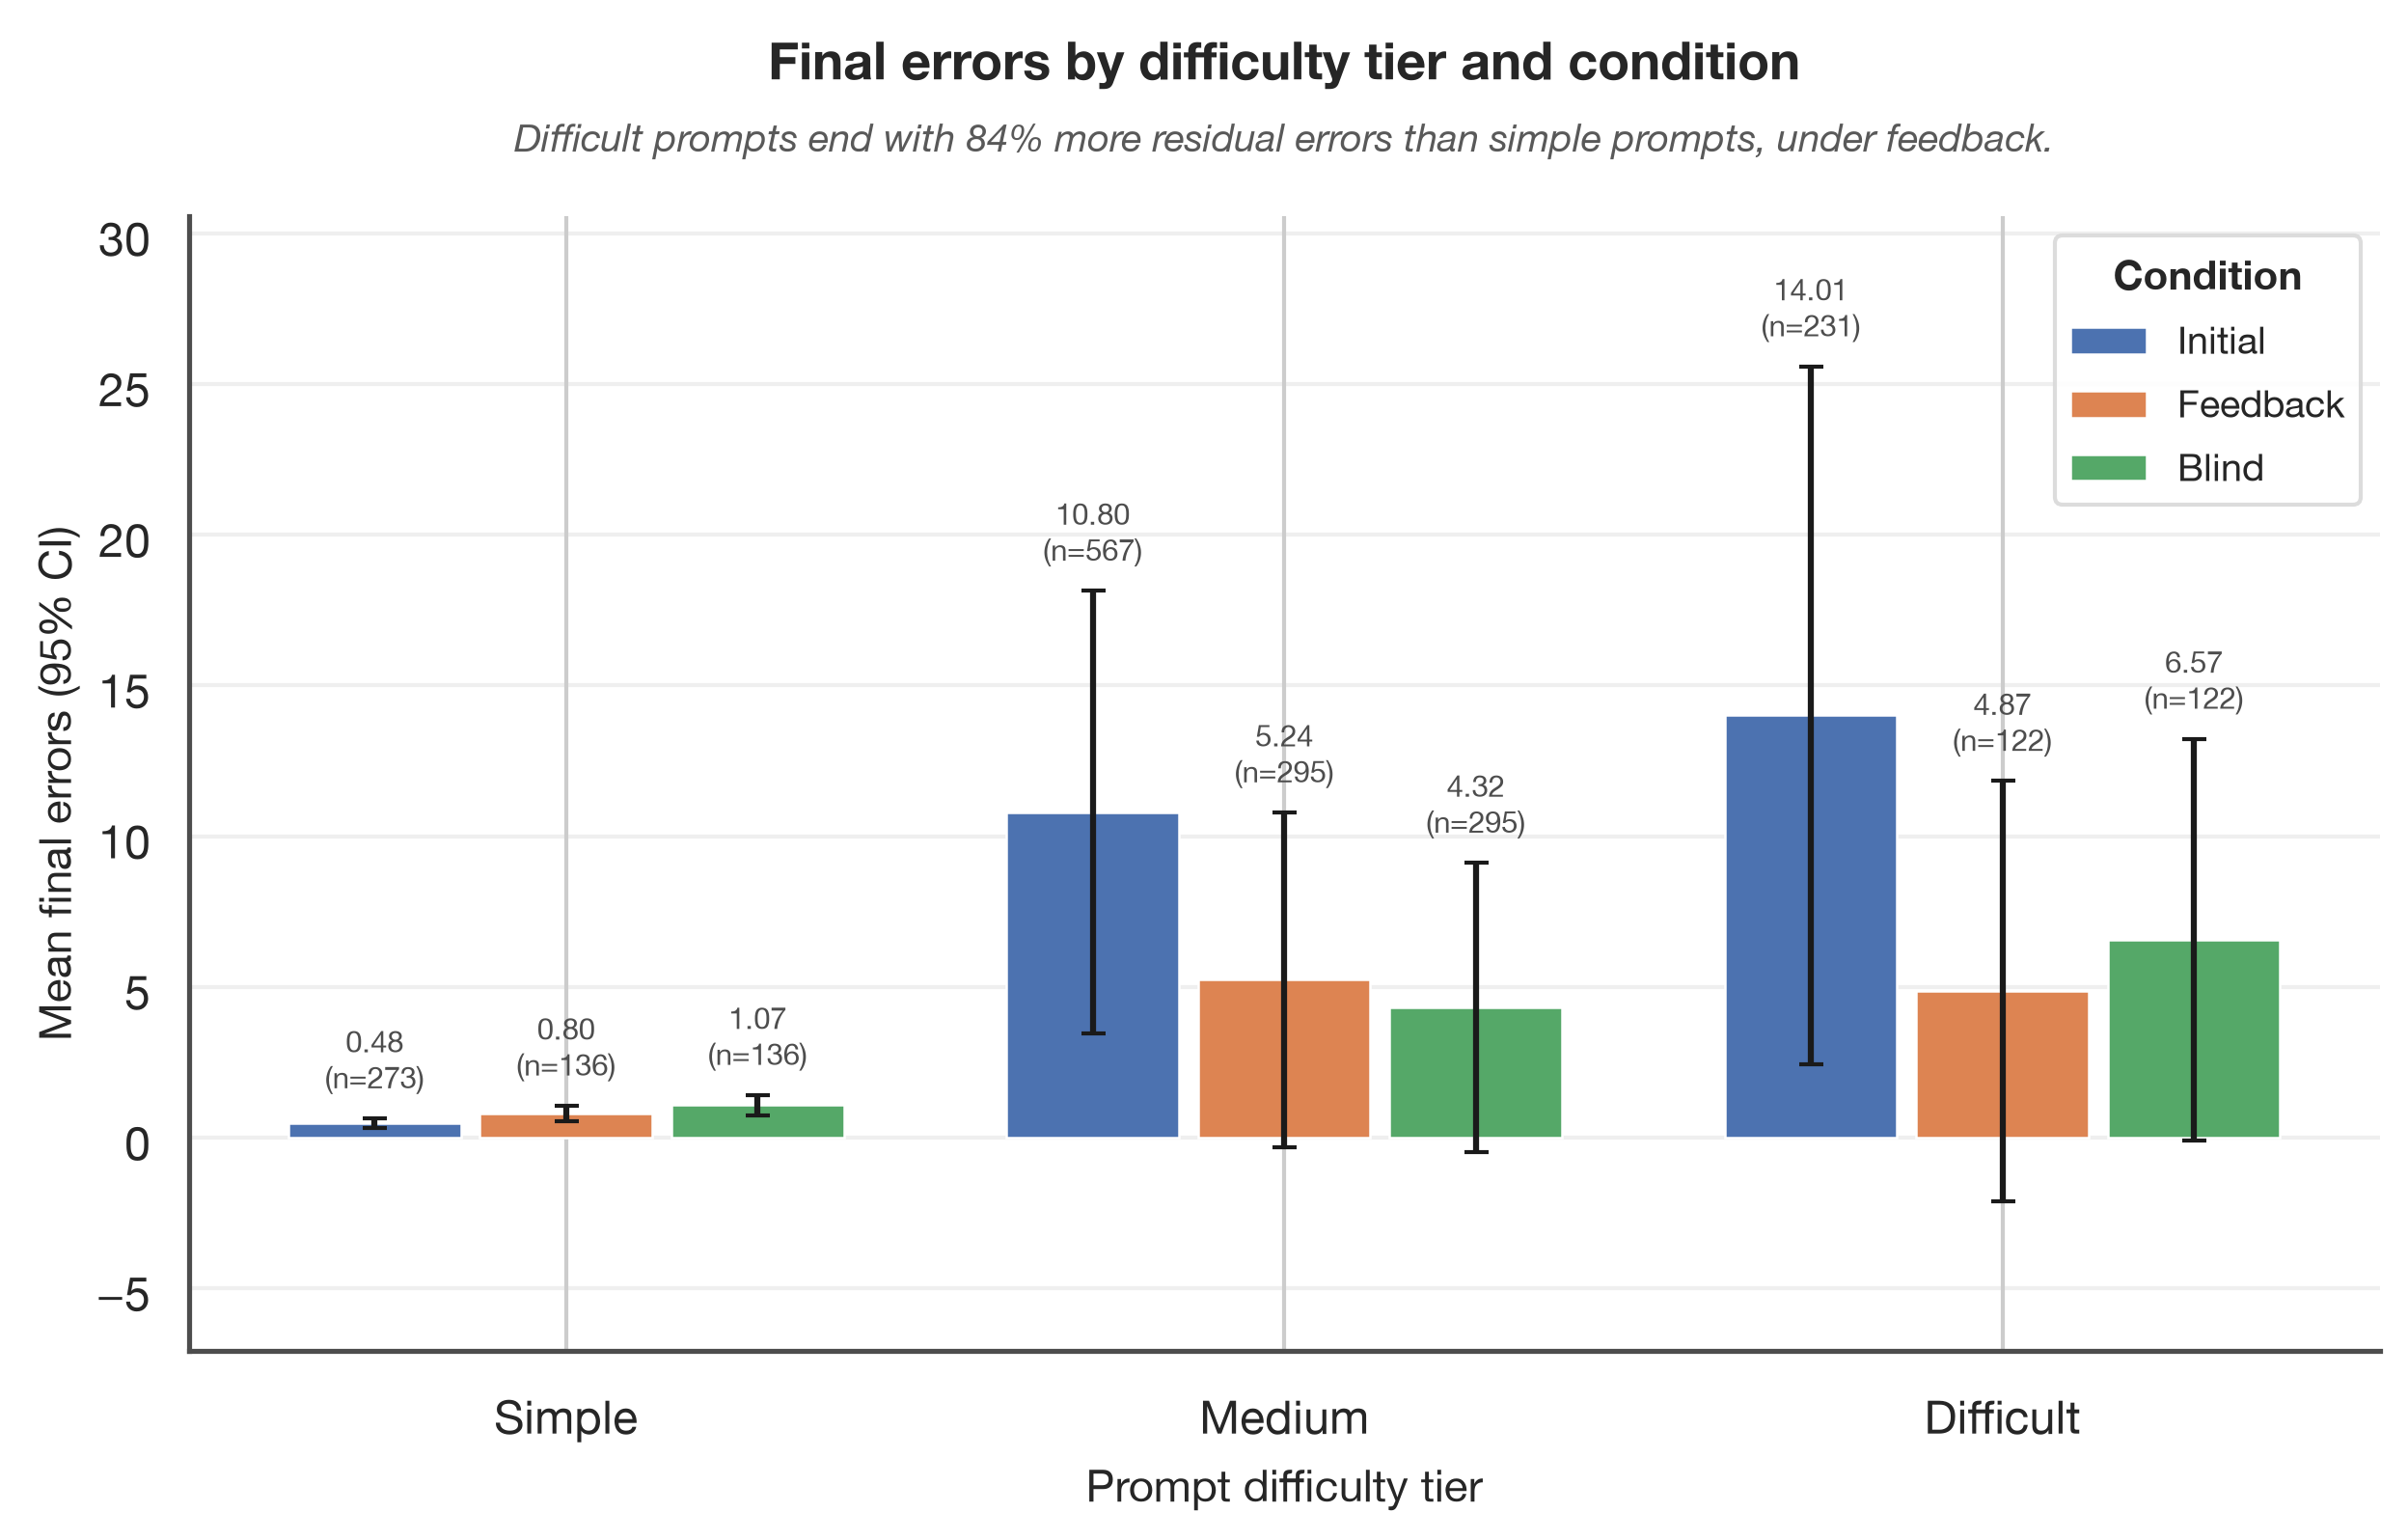
\includegraphics[width=\linewidth]{images/difficulty_tier_errors.png}
	\caption{Mean final error count (95\% CI) by prompt difficulty tier and condition. Value and $n$ are annotated above each bar.}
	\label{fig:difficulty-tier-errors}
\end{figure}

% = PARAGRAPH 5 = Error category breakdown

Discuss which error types the guardrail is most and least effective at resolving. For example: does it reliably fix missing-doctype errors? Does it struggle with disallowed-attribute errors? This dimension answers the qualitative question of what the guardrail actually corrects, and is important for contextualising the aggregate numbers. A small frequency table of error categories (before vs. after) serves this paragraph well. I think I can retrieve this data from the json files in validation/reprompt/, not sure though?

% Answer: the raw per-run validator JSON files aren't checked into the repo (only results/experiments.csv is), but experiments.csv already carries a pre-computed error_categories column per run (from util.validation.categorize_messages), so no JSON parsing is needed -- see analysis.stats.error_category_before_after.
% Error category breakdown table: see tables.tex, Table~\ref{tab:rq1-error-categories} (tab:rq1-error-categories). Note it combines error- and warning-level messages (categorize_messages runs over both), not errors alone -- worth flagging given \S4.4's error/warning distinction.


\subsection{RQ2 \textemdash{} Cost-Efficiency}

% Compare smaller vs. larger models on quality metrics at various iteration counts. Show the quality-vs-cost tradeoff curve. Establish a baseline for large API-based models (or compare against a cited benchmark) as your supervisor suggested.

% \textbf{Change}: Reframe this — the comparison is smaller vs. larger local models only, not local vs. cloud. Add the reasoning vs. non-reasoning dimension as a key finding here, since it turns out to be more predictive of success than parameter count alone. The scatter plots (model size vs. cost/quality, coloured by native thinking mode) directly address this.


% = PARAGRAPH 1 = Framing: what cost-efficiency means here

Briefly restate the scope: this is local-only comparison. Cost is operationalised as generation latency (\verb|gen_time_s|) and token consumption (\verb|prompt_eval_count| + \verb|eval_count|) per run, not API pricing. Set the reader's expectation before presenting numbers

% = PARAGRAPH 2 = Quality vs cost per model

Present the main RQ2 finding: a scatter plot (or table) of each model's error reduction rate against its total generation time and token count. Colour-code or otherwise distinguish reasoning vs non-reasoning models. This is where the core finding lives -- reasoning capability is more predictive of success than parameter count, with \verb|codestral:22b| as the key counterexample (the most parameters, not the absolute best performance due to lack of reasoning -> a smaller model performed ever so slightly better).

\begin{figure}[H]
	\centering
	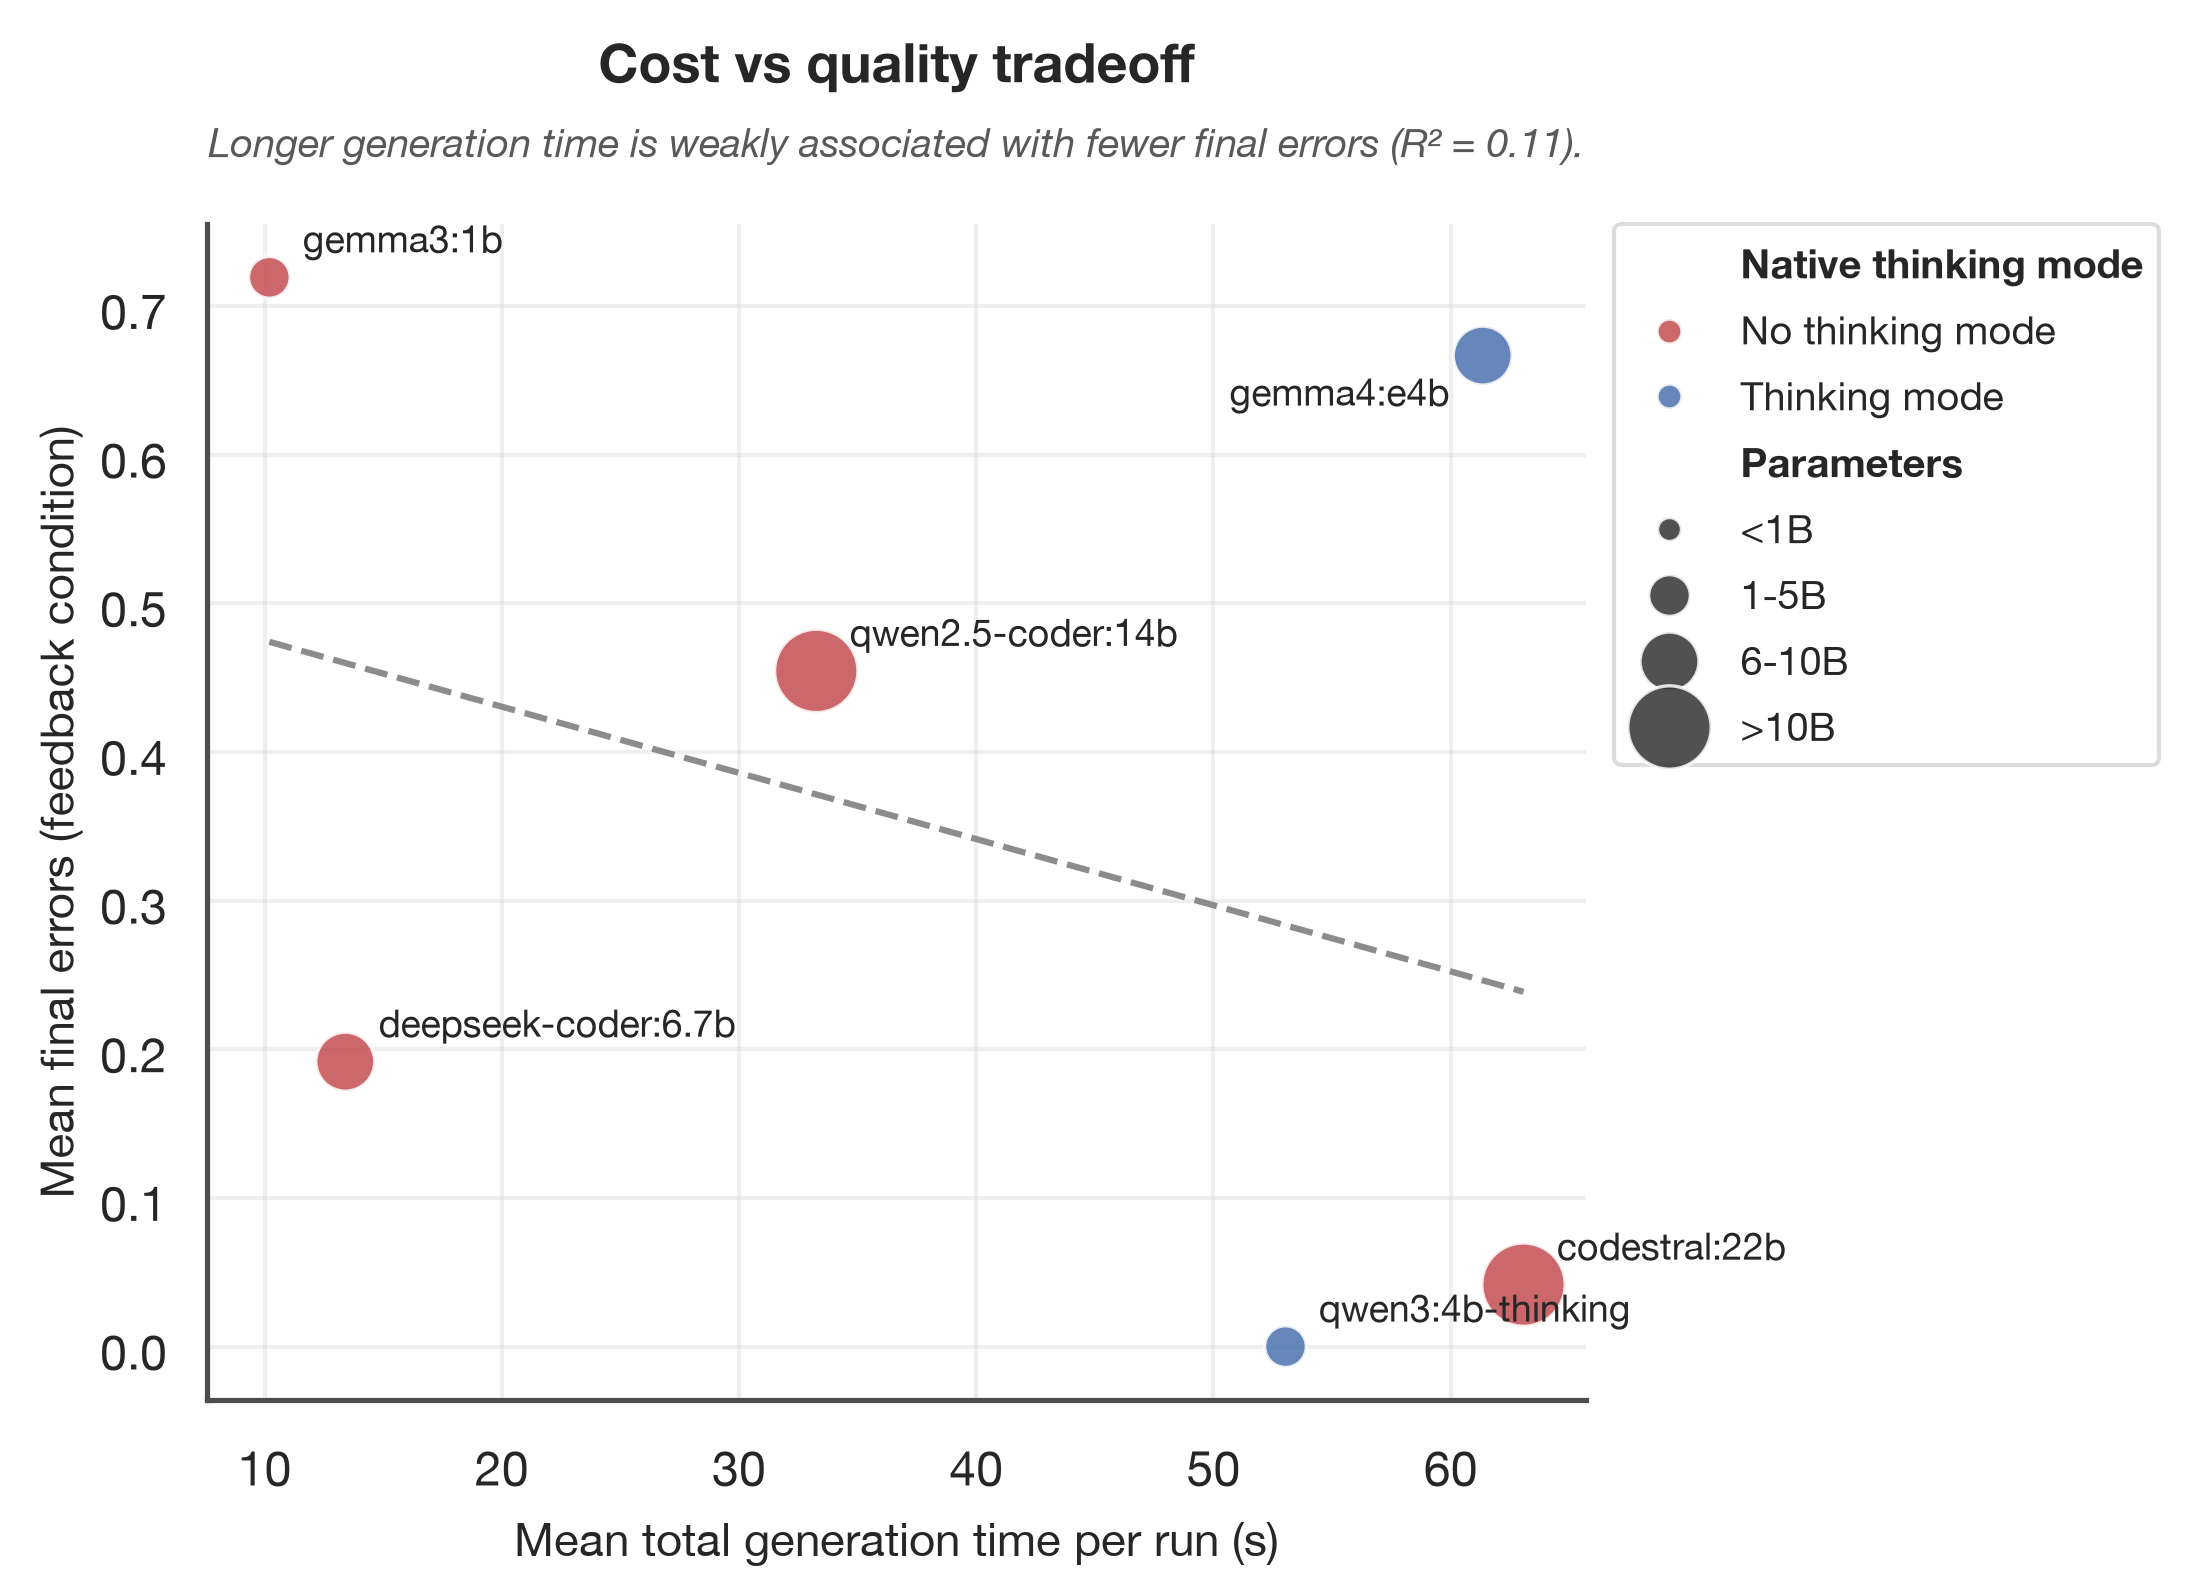
\includegraphics[width=0.85\linewidth]{images/cost_quality_errors.png}
	\caption{Mean total generation time per run vs mean final error count (feedback condition), one point per model. Colour encodes native thinking mode, point size encodes parameter-count bin.}
	\label{fig:cost-quality}
\end{figure}
\begin{figure}[H]
	\centering
	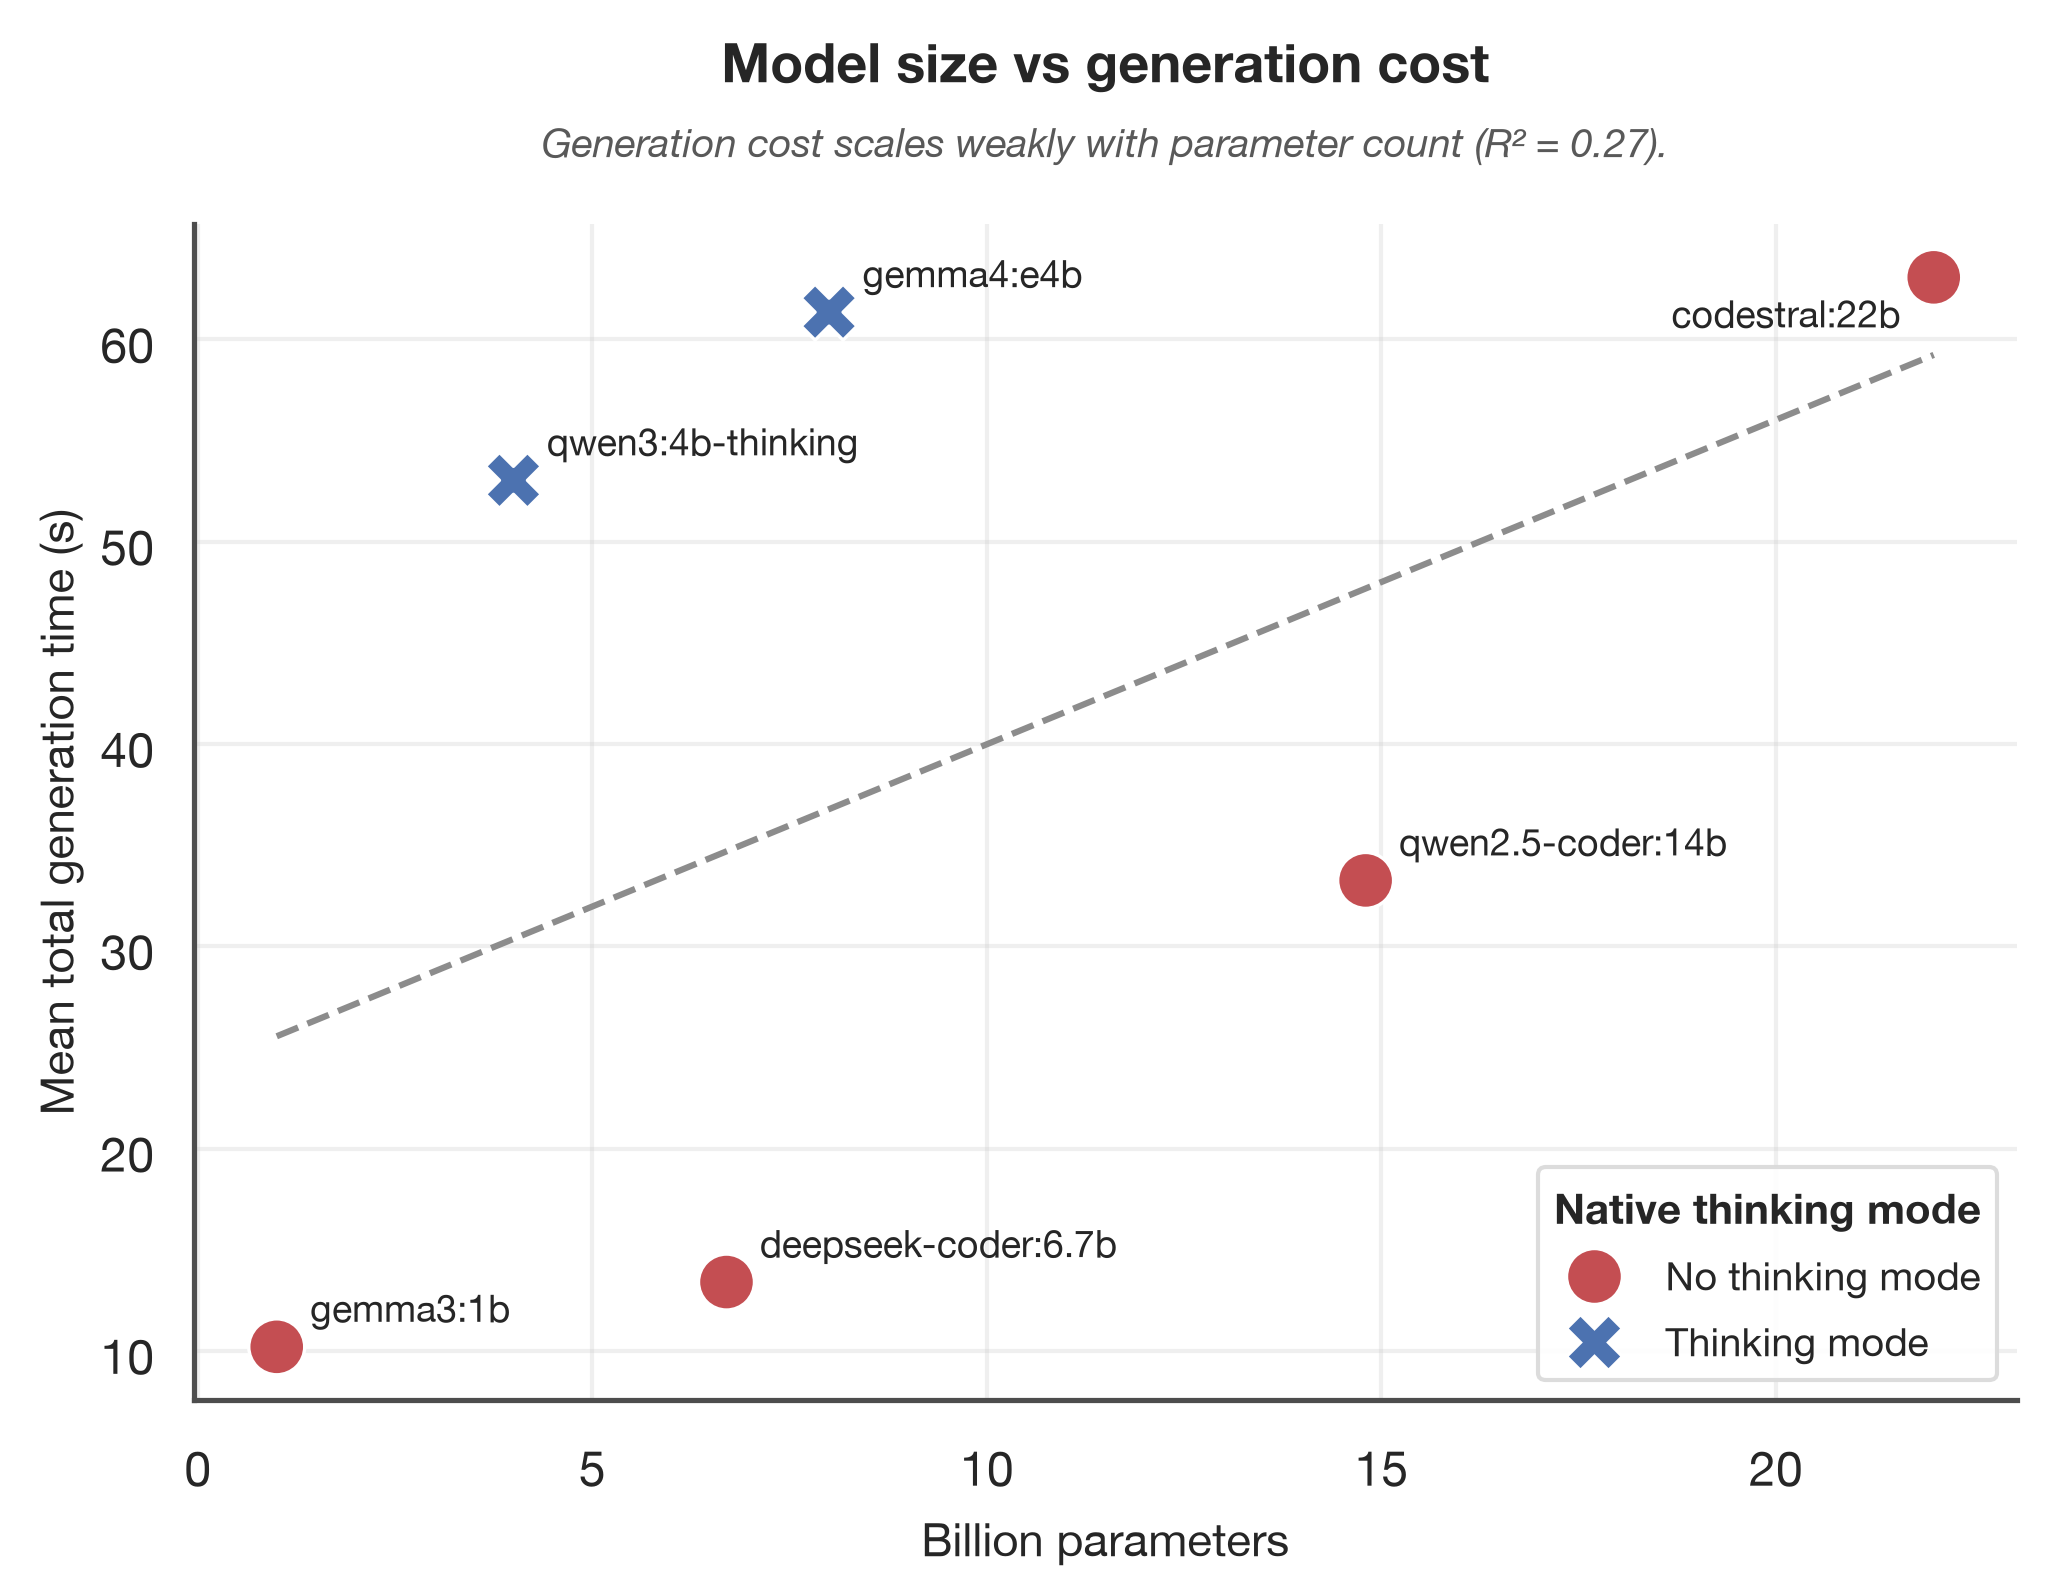
\includegraphics[width=0.7\linewidth]{images/model_size_vs_cost_errors.png}
	\caption{Parameter count vs mean total generation time per run, coloured by native thinking mode.}
	\label{fig:model-size-vs-cost}
\end{figure}

% = PARAGRAPH 3 = Reasoning vs. non-reasoning as the decisive variable

Give this finding its own paragraph because it is the most interesting and surprising result of RQ2. Explicitly compare a smaller reasoning model against codestral:22b. If a reasoning model with fewer parameters achieves better error reduction in fewer iterations at lower latency, that is a concrete, reportable conclusion that directly challenges the assumption that more parameters equal better output.

\begin{figure}[H]
	\centering
	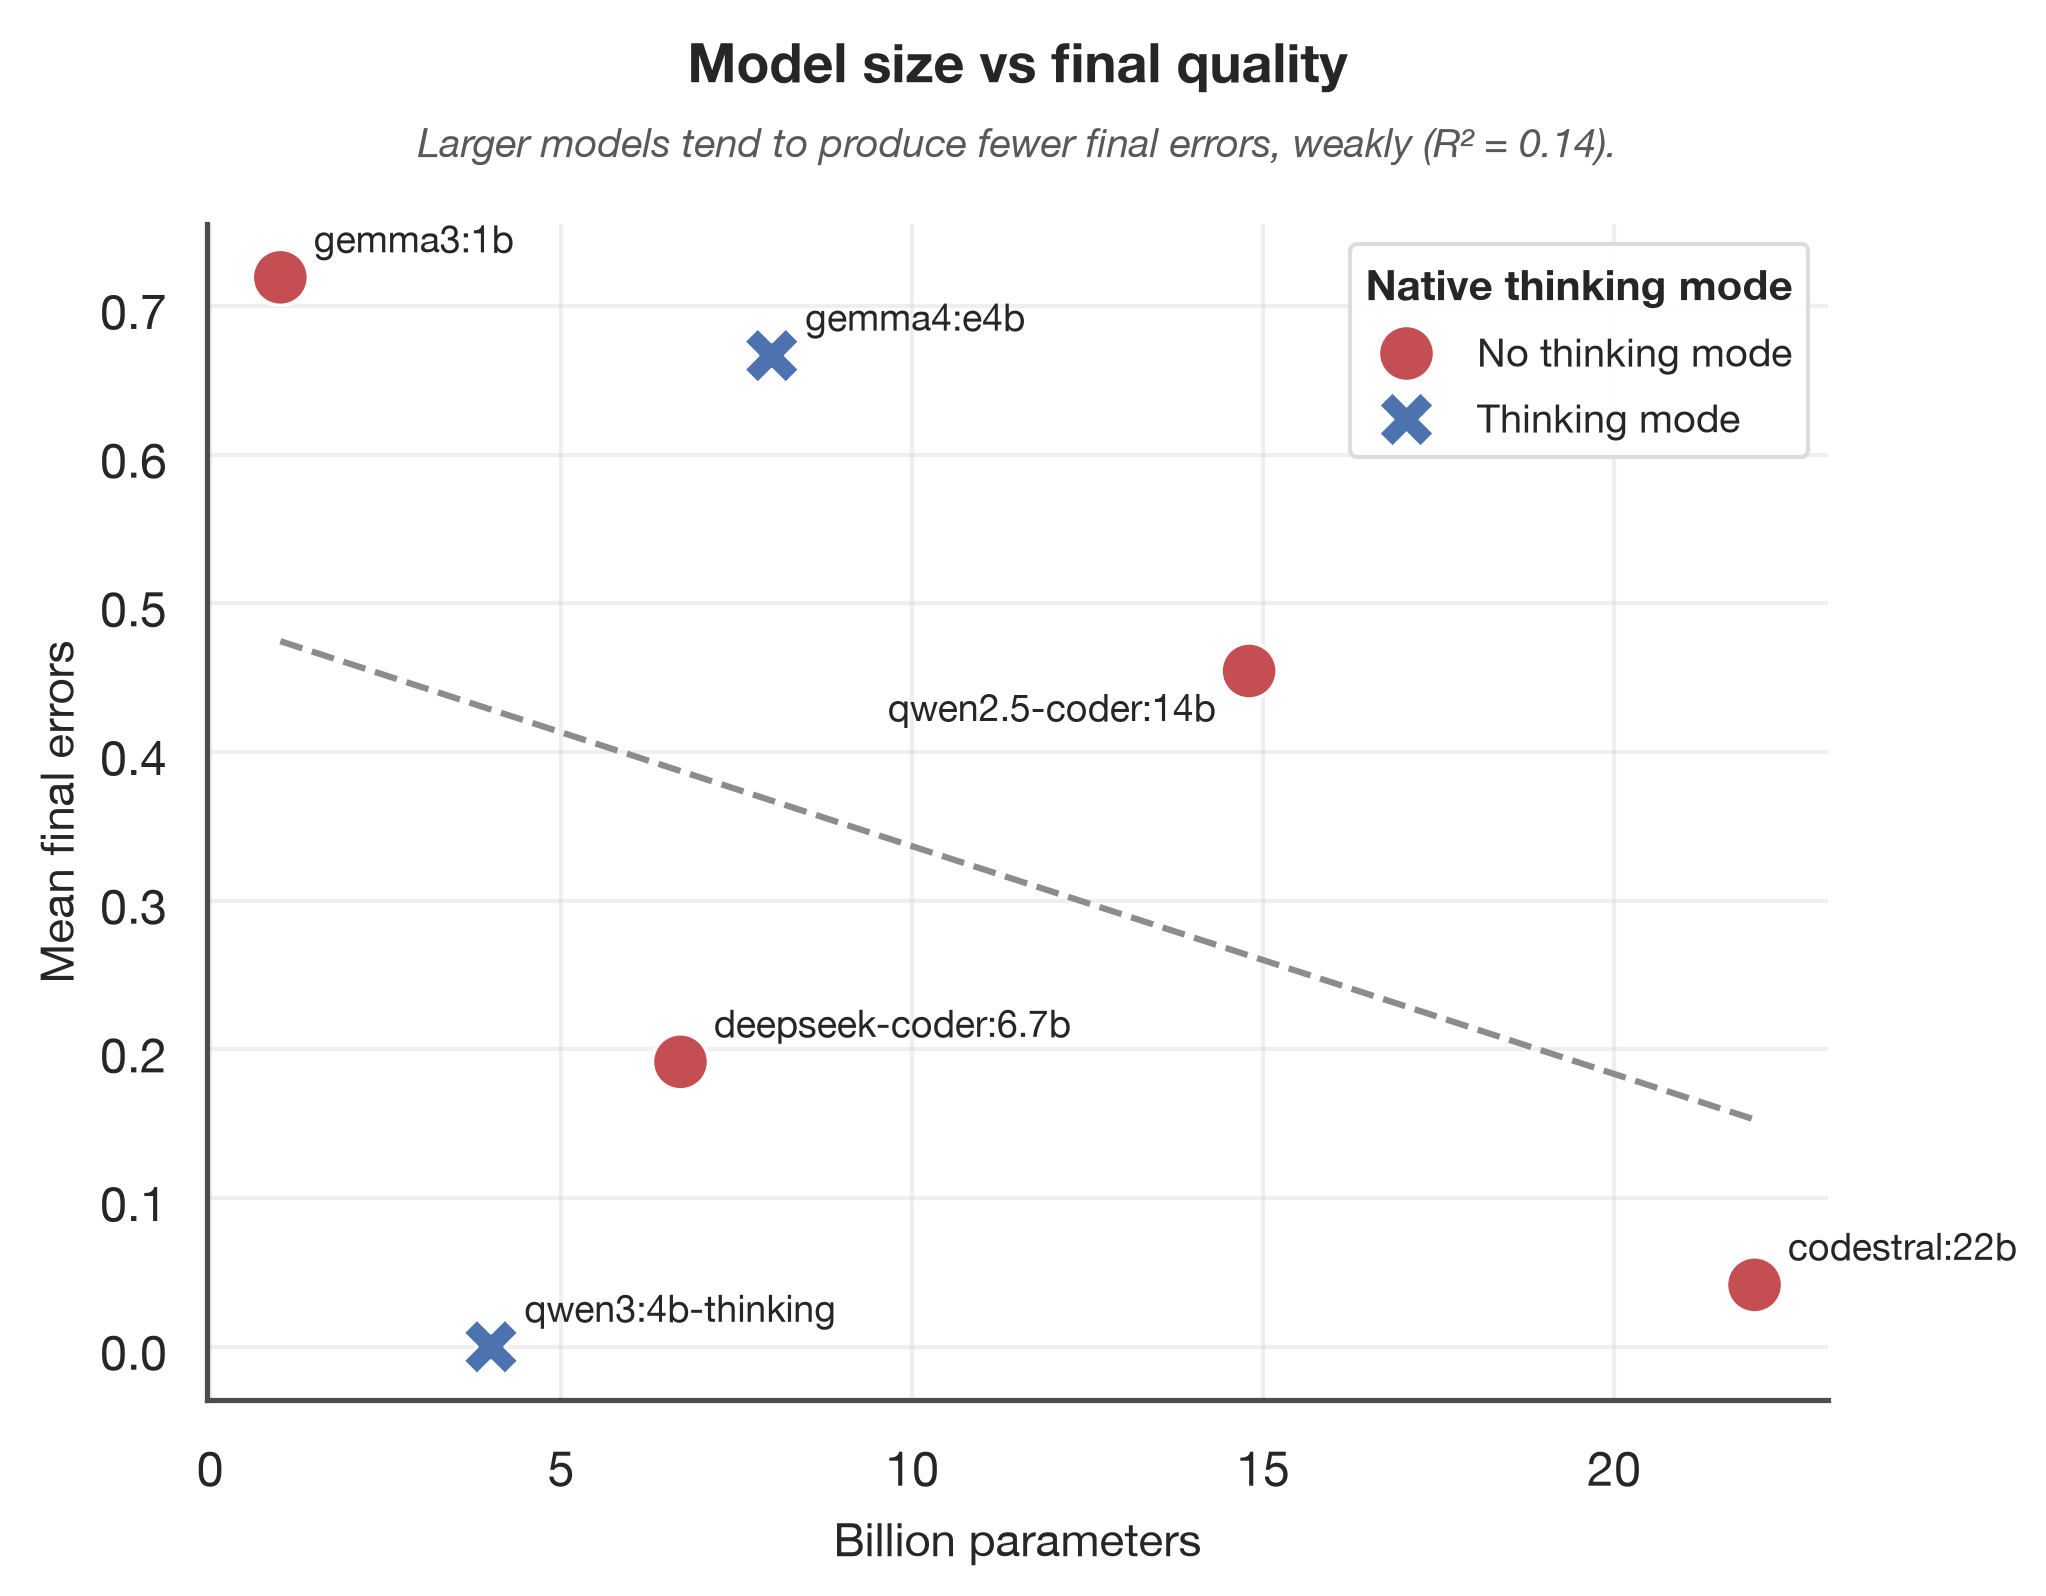
\includegraphics[width=0.7\linewidth]{images/model_size_vs_quality_errors.png}
	\caption{Parameter count vs mean final error count (feedback condition), coloured by native thinking mode. qwen3:4b-thinking (4B, reasoning) reaches a lower mean final error count than codestral:22b (22B, non-reasoning) at roughly a fifth of the parameters.}
	\label{fig:model-size-vs-quality}
\end{figure}

% = PARAGRAPH 4 = Cost of the feedback loop vs. the blind condition

Does the \verb|feedback| condition cost more than \verb|blind| in token terms? It should, since it passes longer prompts (original code + error list). Is the extra cost justified by the quality gain? Frame this as a cost-benefit ratio: additional tokens spent per additional error resolved.

% Answer worth checking before writing this paragraph: per analysis.stats.token_cost_comparison, feedback is actually CHEAPER than blind in total tokens per run for 5 of 7 models (and pooled across all models) -- not more expensive as assumed above. This is because blind converges more slowly (more reprompt iterations needed on average, each carrying its own token cost), so even though each individual feedback iteration's prompt is longer (original code + specific error list), feedback needs fewer of them. Confirm this holds before writing the "it should cost more" framing as-is.
% Cost-benefit table: see tables.tex, Table~\ref{tab:rq2-token-cost} (tab:rq2-token-cost).



\subsection{Iteration Count Analysis}

% When does the loop converge? Is there a diminishing return after N iterations? This is where you answer the "optimal number of iterations" question.

% \textbf{Change}: No major structural change, but the analysis now comes from \verb|stats.py|'s iteration-cutoff analysis, which is worth naming explicitly as the source of the convergence findings.

% = PARAGRAPH 1 = Convergence behaviour

Using the output of \verb|stats.py|'s iteration-cutoff analysis, describe when models typically converge. Do most runs resolve within 1-2 iterations, or does error reduction continue meaningfully up to the maximum? Present a distribution (histogram or line chart) of iterations-to-convergence across all (model, prompt) pairs in the \verb|feedback| condition.

\begin{figure}[H]
	\centering
	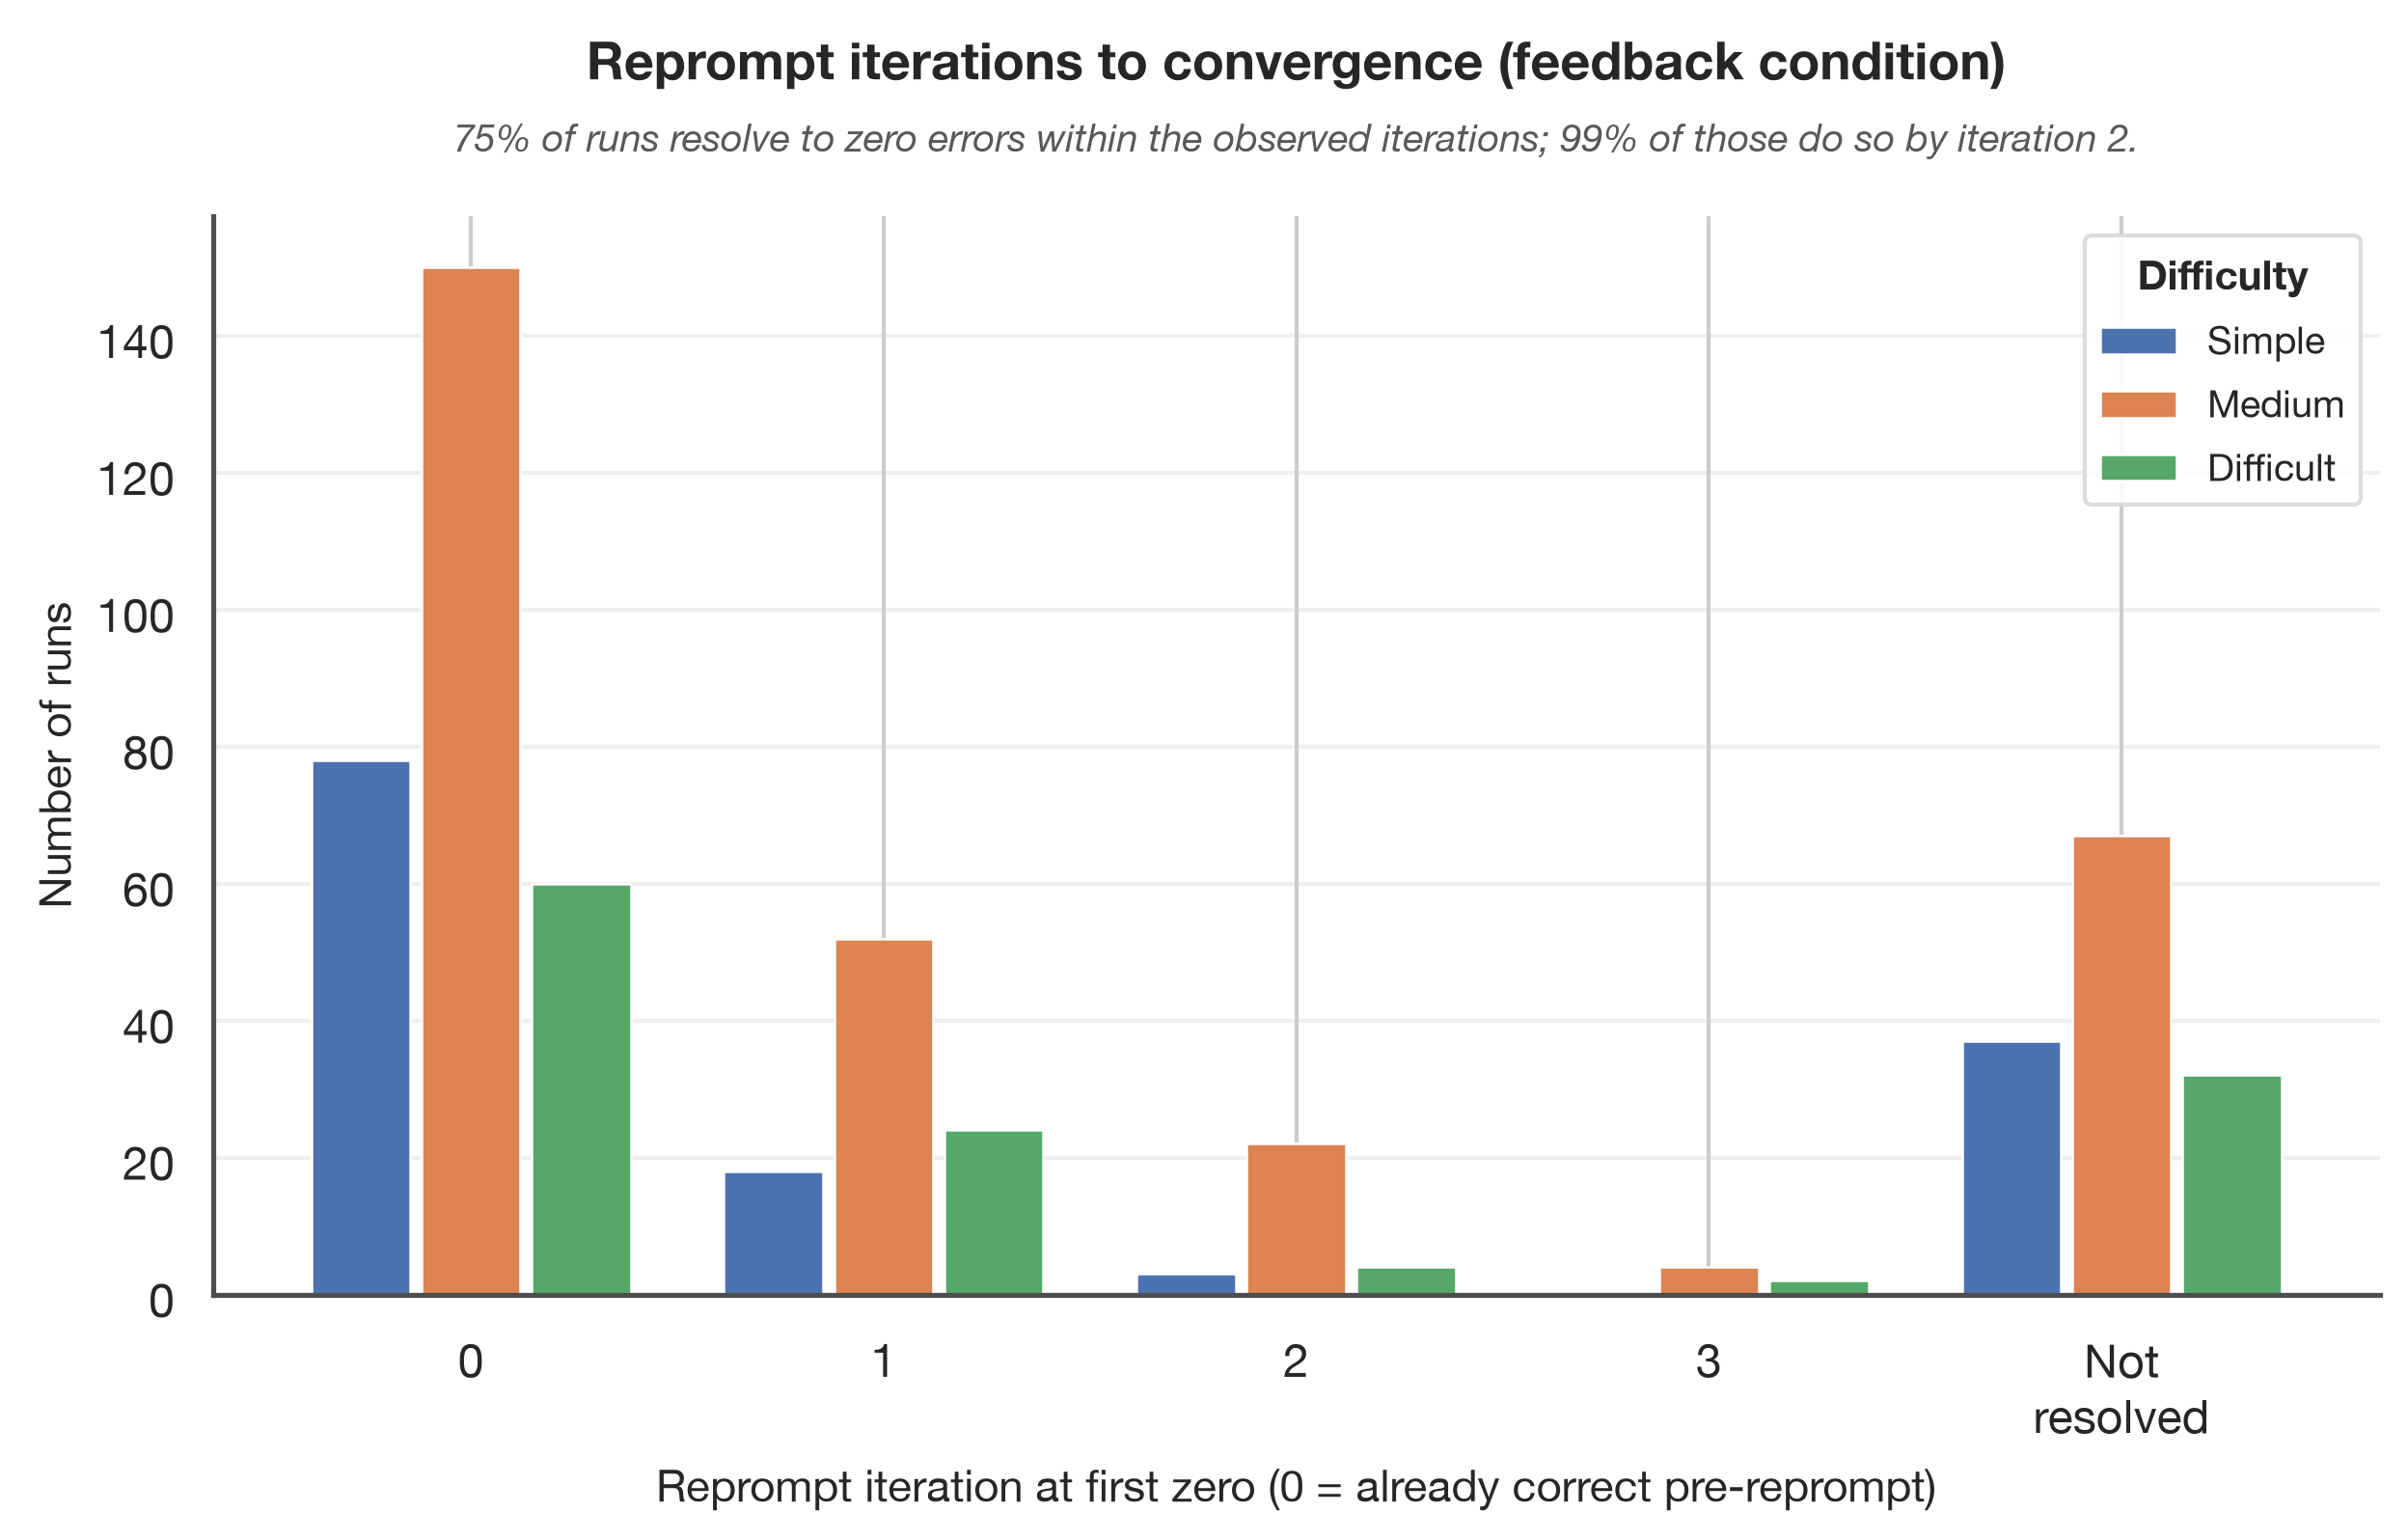
\includegraphics[width=\linewidth]{images/iteration_convergence_errors.png}
	\caption{Distribution of the reprompt iteration at which each (model, prompt, trial) run first reaches zero errors, feedback condition, split by prompt difficulty tier. ``Not resolved'' = still nonzero at the last observed iteration.}
	\label{fig:iteration-convergence}
\end{figure}

% = PARAGRAPH 2 = Dimishing returns and the optimal cut-off

Identify where the marginal gain per additional iteration drops below a meaningful threshold. If, for example, 80\% of resolvable errors are fixed by iteration 2 and iterations 3-5 contribute minimally, that is your practical recommendation for the maximum iteration count. State this as a concrete finding rather than a vague observation. Note whether this threshold differs by model or difficulty tier.

% Cutoff-by-difficulty table: see tables.tex, Table~\ref{tab:iteration-cutoff-difficulty} (tab:iteration-cutoff-difficulty). Per-model cutoff table is the same function with group_by="model" (not pre-generated into tables.tex since it has one row per model per cutoff -- regenerate via analysis.stats.iteration_cutoff_analysis if you want it tabulated too).